\title{Homework 1 Solutions for Computer Logic and Circuit Design: PHYS306/COSC330}
\author{Dr. Jordan Hanson - Whittier College Dept. of Physics and Astronomy}
\date{\today}
\documentclass[10pt]{article}
\usepackage[a4paper, total={18cm, 27cm}]{geometry}
\usepackage{graphicx}
\begin{document}
\maketitle

\section{1-2: Binary Digits, Logic Levels, and Digital Waveforms}

\begin{enumerate}
\item Exercise 7: a) 0.6 $\mu$s, from 0.2 to 0.8 $\mu$s.  Remeber the convention is 10-90 percent of the amplitude. b) 0.55 $\mu$s.  c) 2.7 $\mu$s.  d) 10 V.
\begin{figure}[ht]
\centering
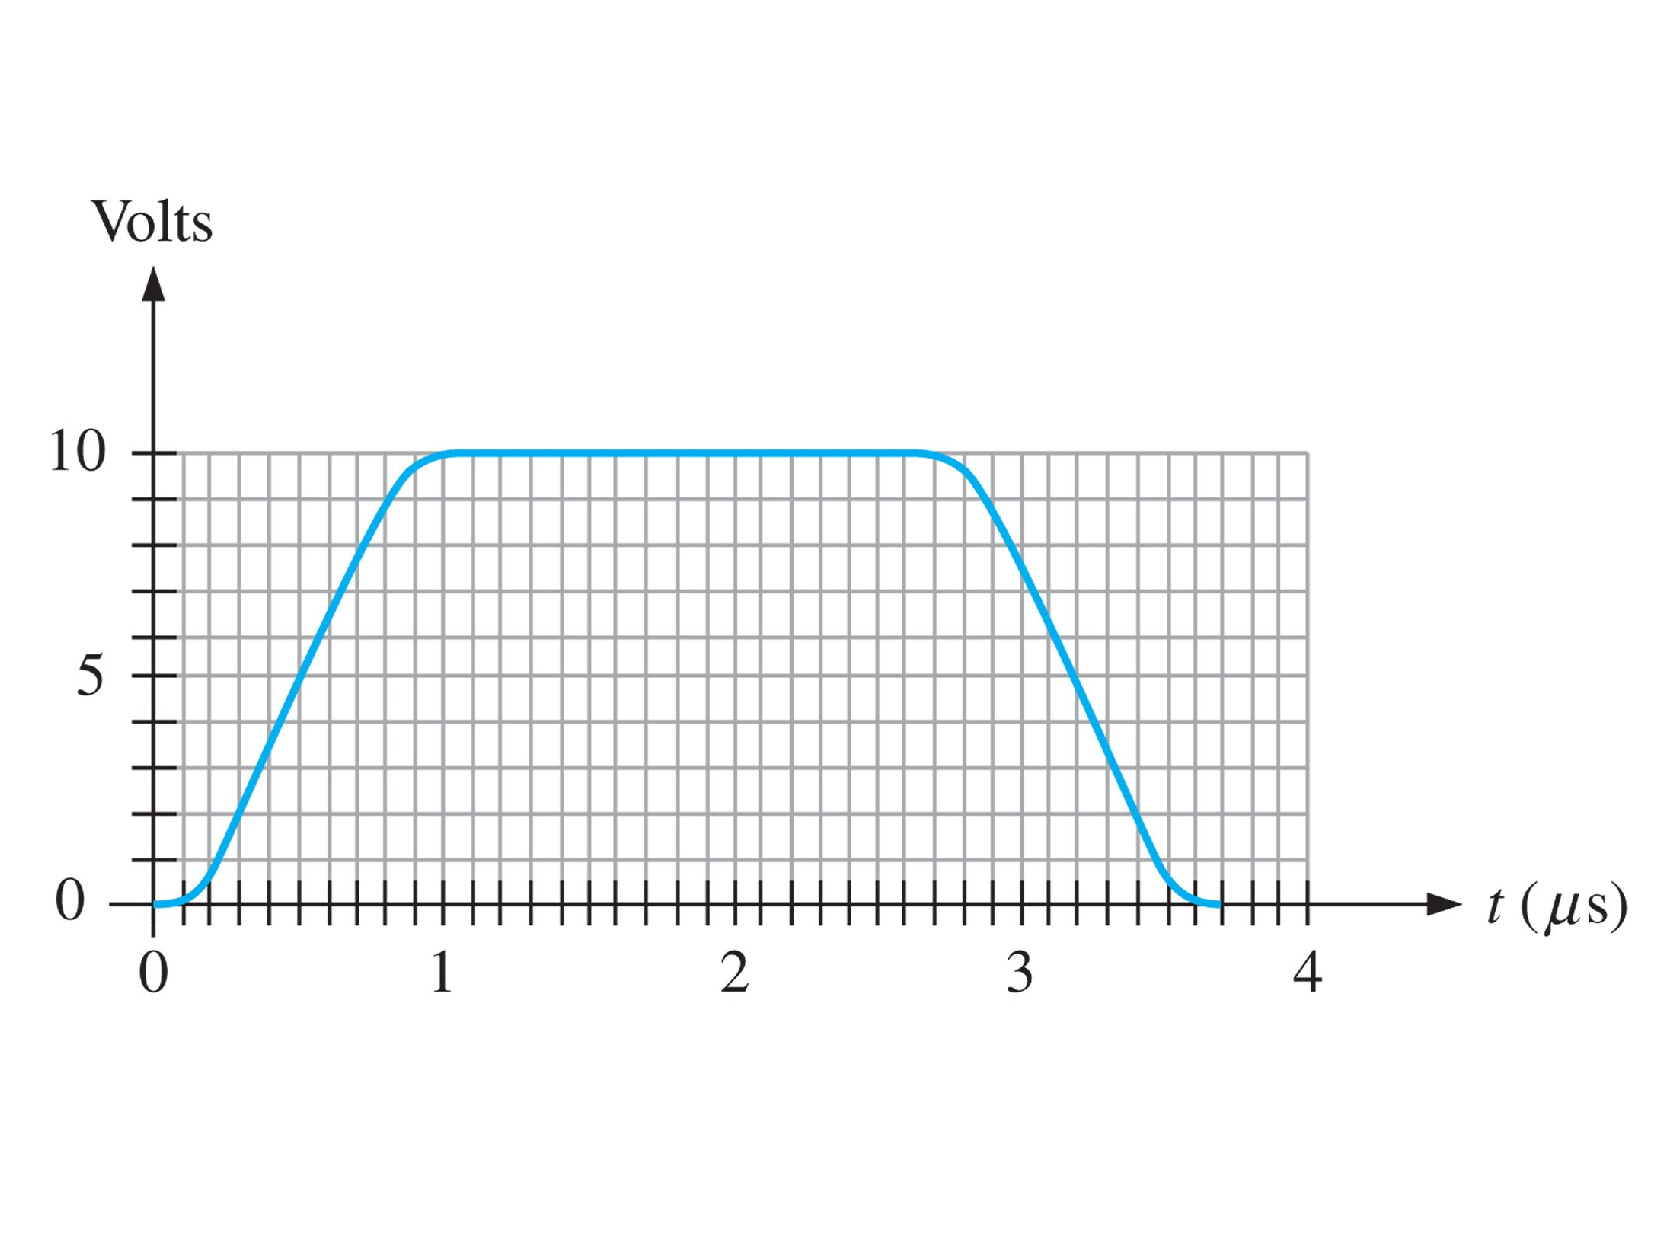
\includegraphics[width=0.3\textwidth,trim=0cm 2cm 0cm 2cm,clip=true]{logicPulse1.pdf}
\caption{\label{fig:logicPulse1} The digital pulse for exercise 7.}
\end{figure}
\item Exercise 8: The period is 4 ms.
\item Exercise 9: The frequency is the inverse of the period, so 0.25 kHz.
\begin{figure}[ht]
\centering
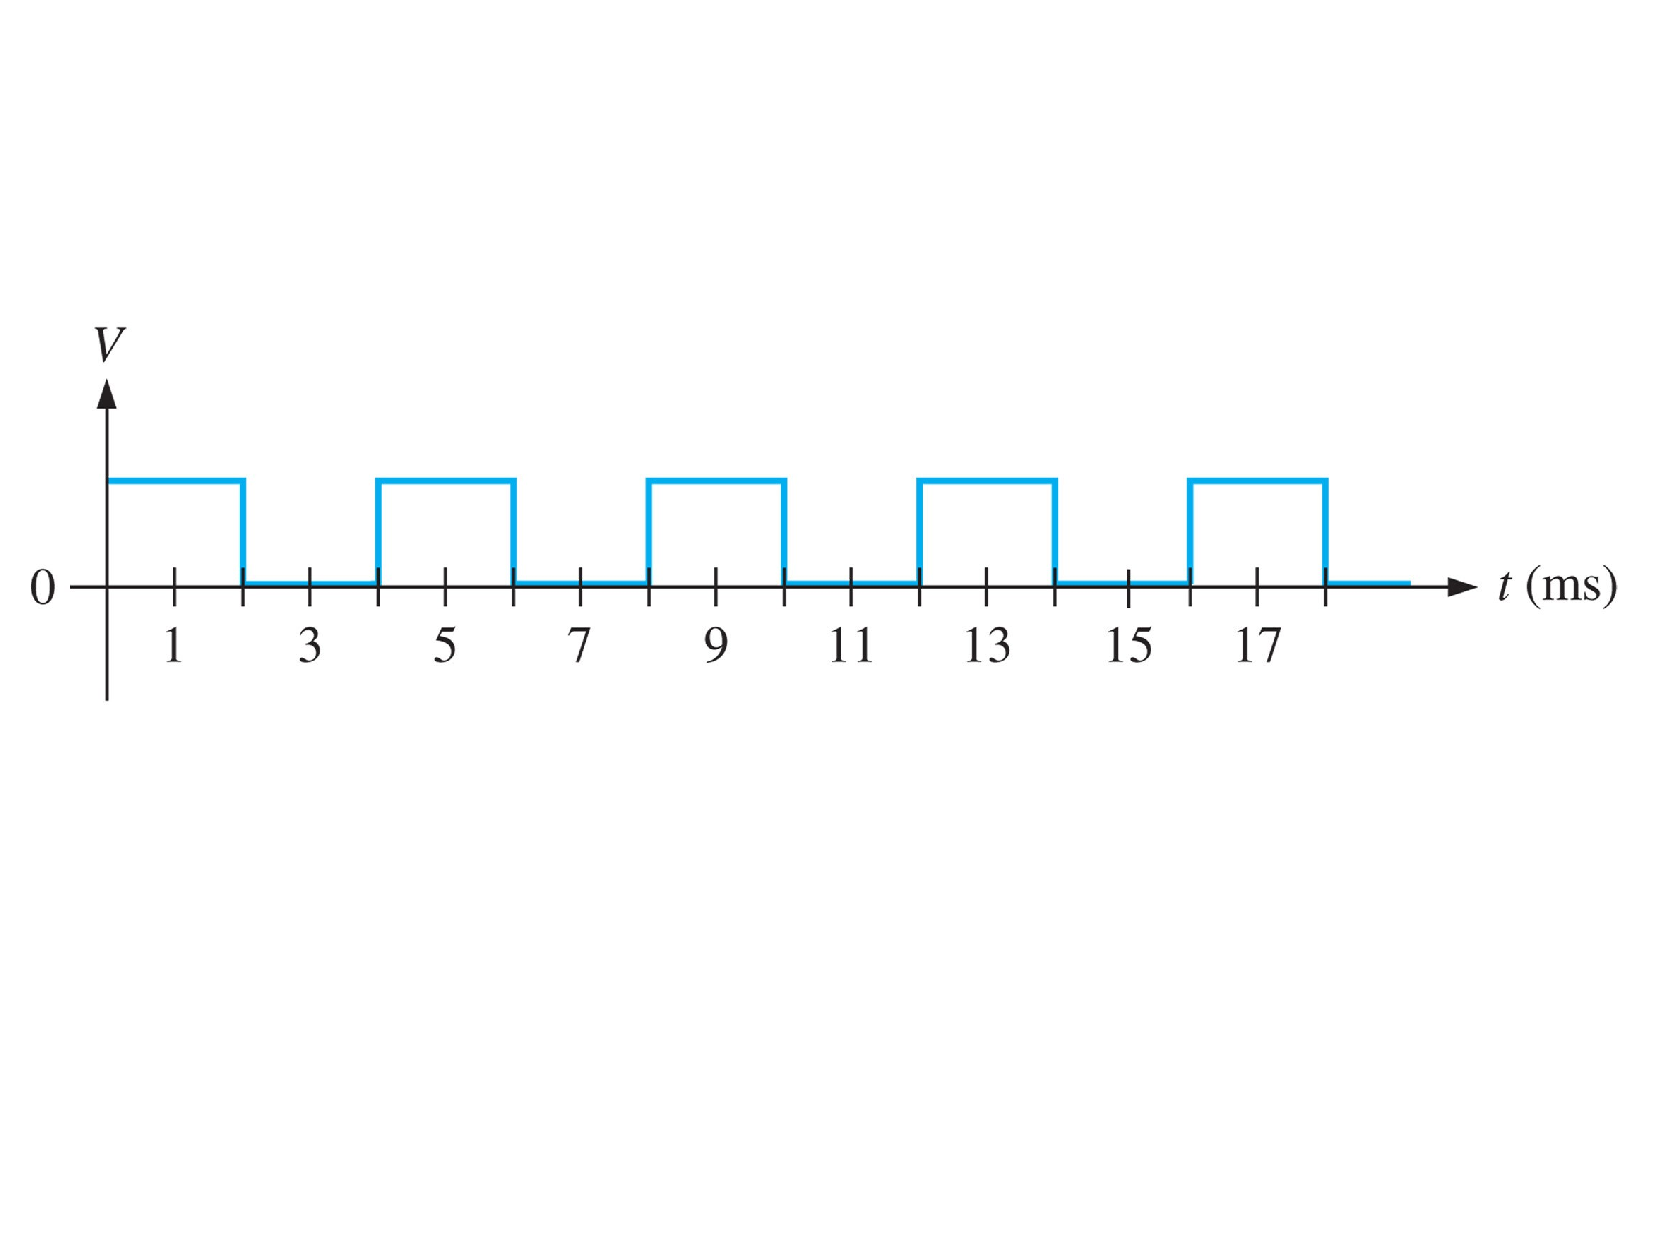
\includegraphics[width=0.4\textwidth,trim=0cm 6cm 0cm 6cm,clip=true]{logicPulse2.pdf}
\caption{\label{fig:logicPulse2} The bitstream/timing diagram for exercise 8.}
\end{figure}
\item Exercise 10: This is an example of a periodic signal.  (\textit{It's a clock signal}).
\item Exercise 11: The duty cycle is 50\%.  The pulse width is 2 ms and the period is 4 ms so the ratio is one-half.
\item Exercise 14: The period is the inverse of the frequency, so $10/35$ ns, or 0.286 ns.
\end{enumerate}

\section{1-3: Basic Logic Functions}

\begin{enumerate}
\item Exercise 15: We have to account for all the information, so the best answer is $LD0 = SW1 ~ | ~ SW2$.  That is $LD0 = SW1$ OR $SW2$.
\end{enumerate}

\section{1-7: Test and Measurement Instruments}

\begin{enumerate}
\item Exercise 30: This is like a units problem, $2 V/div \times 3 div = 6 V$.
\item Exercise 31: This is like a units problem, $2 ms/div \times 4 div = 8 ms$.
\item Exercise 32: This is like a units problem, $12 MS/s \times 2 ms = 12 \times 10^{6} \times 10^{-3} = 24,000$ samples.
\end{enumerate}

\section{2-2: Binary Numbers}

\begin{enumerate}
\item Exercise 6: Convert the following binary numbers to decimal:
\begin{itemize}
\item (a) 14
\item (b) 10
\item (c) 28
\item (d) 16
\item (e) 21
\item (f) 29
\item (g) 23
\item (h) $31 \rightarrow 2^5 - 1$
\end{itemize}
\end{enumerate}

\section{2-4: Binary Arithmetic}

\begin{enumerate}
\item Exercise 15:
\begin{itemize}
\item (a) 100 (4)
\item (b) 100 (4)
\item (c) 1000 (8)
\item (d) 1101 (13)
\item (e) 1110 (14)
\item (f) 11000 (24)
\end{itemize}
\item Exercise 17:
\begin{itemize}
\item (a) 1001 (9)
\item (b) 1000 (8)
\item (c) 100011 (35)
\item (d) 110110 (58)
\item (e) 1010 1001 (169) ... with this number of total bits, verify in decimal (1101 = 13, 13 x 13 = 169)
\item (f) 1011 0110 (182) ... (14 x 13 = 182)
\end{itemize}
\end{enumerate}

\end{document}
